\subsection{The implications of a gravitational potential not from the space of model potentials} \label{sec:results_potential}

%Motivation for the Test

We now explore what happens when the mock data were drawn from one axisymmetric potential family, here \texttt{MW14-Pot}, and is then modelled considering potentials from only another axisymmetric family, here \texttt{KKS-Pot} (see Table \ref{tbl:referencepotentials} and Figure \ref{fig:ref_pots}). In the analysis we assume the circular velocity at the Sun to be fixed and known and only fit the parametric potential form. 

%====================================================================

\begin{figure}[!htbp]
\plotone{figs/MW14vsKKS2SphFlex_mockdata_residuals_2.eps}
\caption{Comparison of the distribution of mock data in configuration space created in the \texttt{MW14-Pot} potential and with two different stellar populations (see Test \ref{test:MW14vsKKS2SphFlex} in Table \ref{tbl:tests} for all mock data model parameters), and the best fit distribution recovered by fitting the family of \texttt{KKS-Pot} potentials to the data. The best fit potentials are shown in Figure \ref{fig:MW14vsKKS2SphFlex} and the corresponding best fit qDF parameters in Figure \ref{fig:MW14vsKKS2SphFlex_violins}. The data is very well recovered, even though the fitted potential family did not incorporate the true potential. \Wilma{[TO DO: $\text{km s}^{-1}$ and $\text{mas yr}^{-1}$]}}
\label{fig:MW14vsKKS2SphFlex_mockdata_residuals}
\end{figure}

\begin{figure*}[!htbp]
\centering
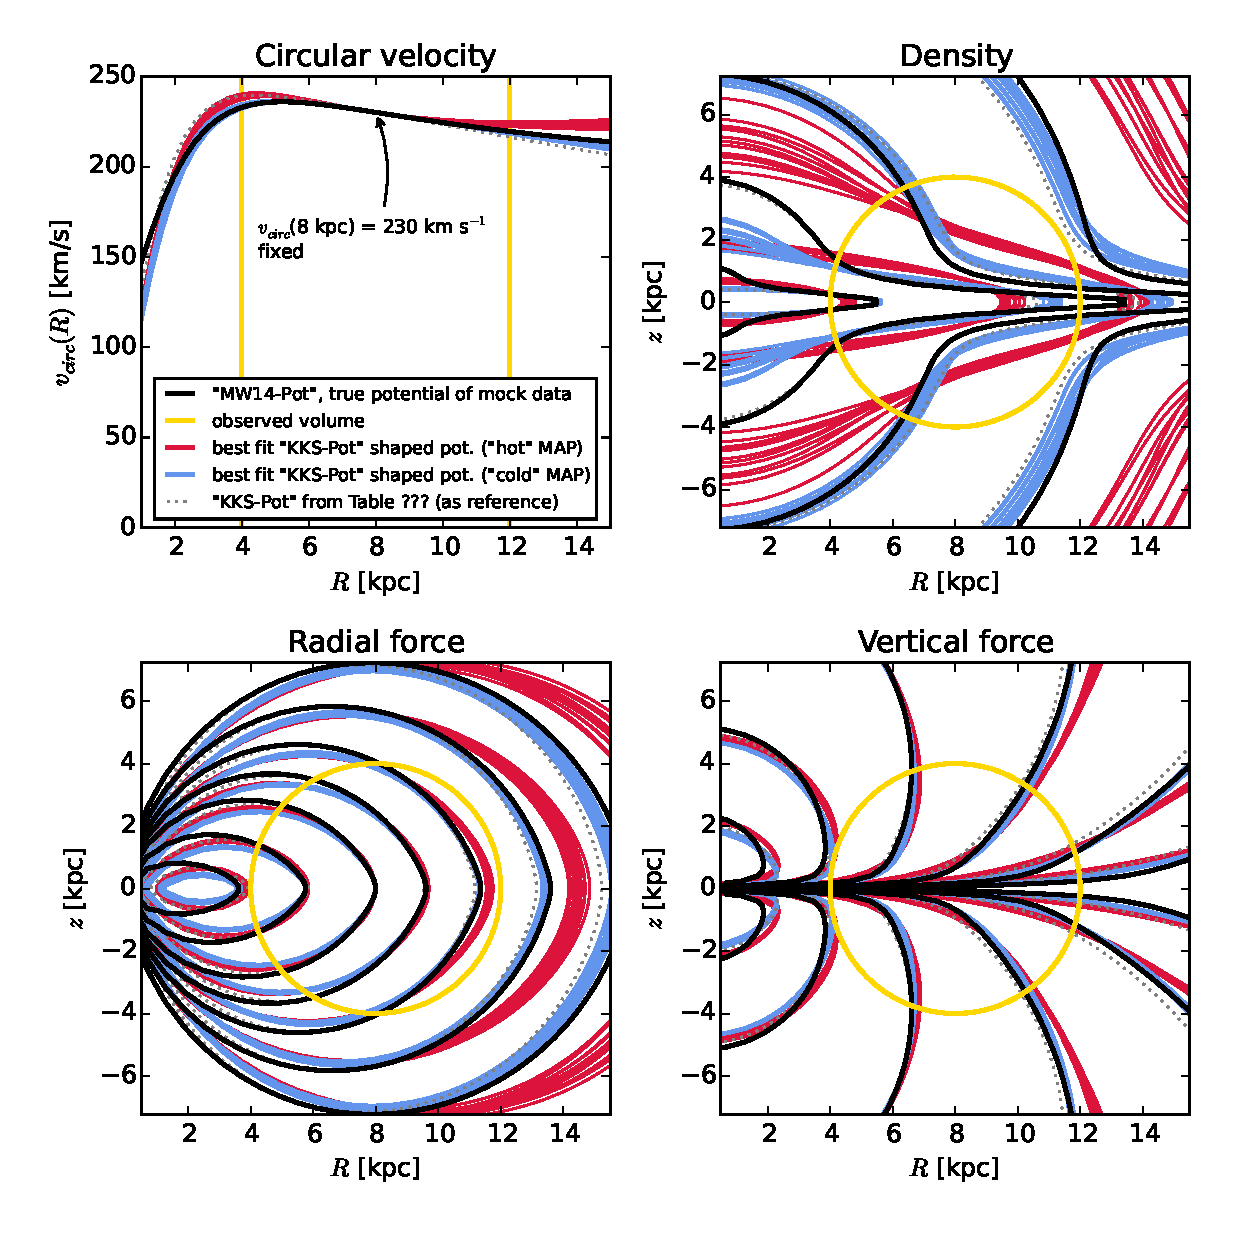
\includegraphics[width=0.7\textwidth]{figs/MW14vsKKS2SphFlex_contours_compare.eps}
\caption{Recovery of the gravitational potential if the assumed potential model (\texttt{KKS-Pot} with fixed $v_\text{circ}(R_\odot)$) and the true potential of the (mock data) stars (\texttt{MW14-Pot} in Table \ref{tbl:referencepotentials}) are slightly different. We show the circular velocity curve, as well as contours of equal density, radial and vertical force in the $R$-$z$-plane, and compare the true potential with 100 sample potentials drawn from the\pdf{} found with the MCMC for a \texttt{hot} (red) and a \texttt{cool} stellar population (blue). (All model parameters are given as Test \ref{test:MW14vsKKS2SphFlex} in Table \ref{tbl:tests}.) \Wilma{[TO DO: Do more analyses???] [TO DO: Reference correct Table in Plot - don't forget!] [TO DO: Redo whole analysis with vcirc not being fixed (HW is not sure if this really doesn't make a difference.] [TO DO: MEntion that high precision is needed.]}}
\label{fig:MW14vsKKS2SphFlex}
\end{figure*}

\begin{figure*}[!htb]
\plotone{figs/MW14vsKKS2SphFlex_violins.eps}
\caption{Recovery of the qDF parameters for the case where the true and assumed potential deviate from each other (see Test \ref{test:MW14vsKKS2SphFlex} in Table \ref{tbl:tests}). The thick red (blue) lines represent the true qDF parameters of the \texttt{hot} (\texttt{cool}) qDF in Table \ref{tbl:referenceMAPs} used to create the mock data, surrounded by a 10\% error region. The grey violins are the marginalized \pdf{}s for the qDF parameters found simultaneously with the potential constraints shown in Figure \ref{fig:MW14vsKKS2SphFlex}. \Wilma{[TO DO: $\text{km s}^{-1}$ and $\text{mas yr}^{-1}$]}}
\label{fig:MW14vsKKS2SphFlex_violins}
\end{figure*}



%====================================================================


%Results on the potential

We analyse a mock data set from each a \texttt{hot} and \texttt{cool} stellar population (see Test \ref{test:MW14vsKKS2SphFlex} in Table \ref{tbl:tests}). The distributions generated from the best fit parameters reproduce the data in configuration space very well (see Figure \ref{fig:MW14vsKKS2SphFlex_mockdata_residuals}).

The results for the potential are shown in Figure \ref{fig:MW14vsKKS2SphFlex}. We find that the potential recovered by \RM{} is in good agreement with the true potential. Especially the force contours, to which the orbits are sensitive, and the rotation curve are very tightly constrained and reproduce the true potential even outside of the observed volume of the mock tracers.

Overplotted in Figure \ref{fig:MW14vsKKS2SphFlex} is also the \texttt{KKS-Pot} with the parameters from Table \ref{tbl:referencepotentials}, which were fixed based on a (by-eye) fit \emph{directly} to the force field (within $r_\text{max}=4~\text{kpc}$ from the Sun) and rotation curve of the \texttt{MW14-Pot}. The potential found with the \RM{} analysis is an equally good or even slightly better fit. This demonstrates that \RM{} fitting infers a potential that in its actual properties resembles the input potential for the mock data as closely as possible, given the differences in functional forms.

The density contours are less tightly constrained than the forces, but we still capture the essentials. Overall the best fit disk is less dense in the midplane than the true disk, because the generation of very flattened components like exponential disks with St\"{a}ckel potentials is not possible \Wilma{[TO DO: Ask Glenn, if this is true]}.

%Results on the qDF

Figure \ref{fig:MW14vsKKS2SphFlex_violins} compares the true qDF parameters with the best fit qDF parameters belonging to the potentials in Figure \ref{fig:MW14vsKKS2SphFlex}. While we recover $h_R$, $\sigma_{R,0}$ and $h_{\sigma,R}$ within the errors, we misjudge the parameters of the vertical velocity dispersion ($\sigma_{0,z}$ and $h_{\sigma,z}$), even though the actual mock data distribution is well produced. This discrepancy could be connected to the \texttt{KKS-Pot} not being able to reproduce the flattness of the disk. Also, $\sigma_z$ and $\sigma_R$ in Equations \ref{eq:sigmaRRg}-\ref{eq:sigmazRg} are scaling profiles for the qDF (cf. BR13) and how close they are to the actual velocity profile depends on the choice of potential.










